\documentclass[fleqn]{article}
\usepackage[utf8]{inputenc}
\usepackage[T1]{fontenc}
\usepackage[plmath,T1]{polski}
\usepackage{graphicx, mathtools,amsthm,amssymb}
\usepackage[hidelinks]{hyperref}
\usepackage{gensymb}
\usepackage[margin=0.7in]{geometry}
\usepackage{float}
\usepackage{dsfont}
\usepackage{xcolor}
\usepackage{multirow}
\usepackage{multicol}
\usepackage{mdframed}
\usepackage{amsthm}
\theoremstyle{plain}
\newtheorem*{theorem*}{Definicja}

\author{Ada Majchrzak, Aleksander Jakóbczyk}
\title{Komputerowa analiza szeregów czasowych - raport II \\[1ex] \large Analiza danych z wykorzystaniem modeli ARMA}

\begin{document}
    \maketitle

    \section{Wstęp}
    W poniższej pracy zajęliśmy się analizą danych pochodzących ze strony Yahoo Finance:
    \href{https://finance.yahoo.com/quote/EURPLN%3DX/history?p=EURPLN%3DX}{\color{blue} EUR/PLN}. Badane dane pochodzą z okresu od 2017-02-06 do 2022-02-04, zawierają 1305 obserwacji i dotyczą
    kursu euro w stosunku do złotego. Dla niektórych z dni cena nie została określona - w takim przypadku nieznaną cenę zastąpimy średnią z dwóch najbliższych dni.
    Głównym celem raportu będzie konstrukcja modelu ARMA, estymacja jego parametrów oraz analiza residuów. 
    \begin{figure}[H]
        \centering
        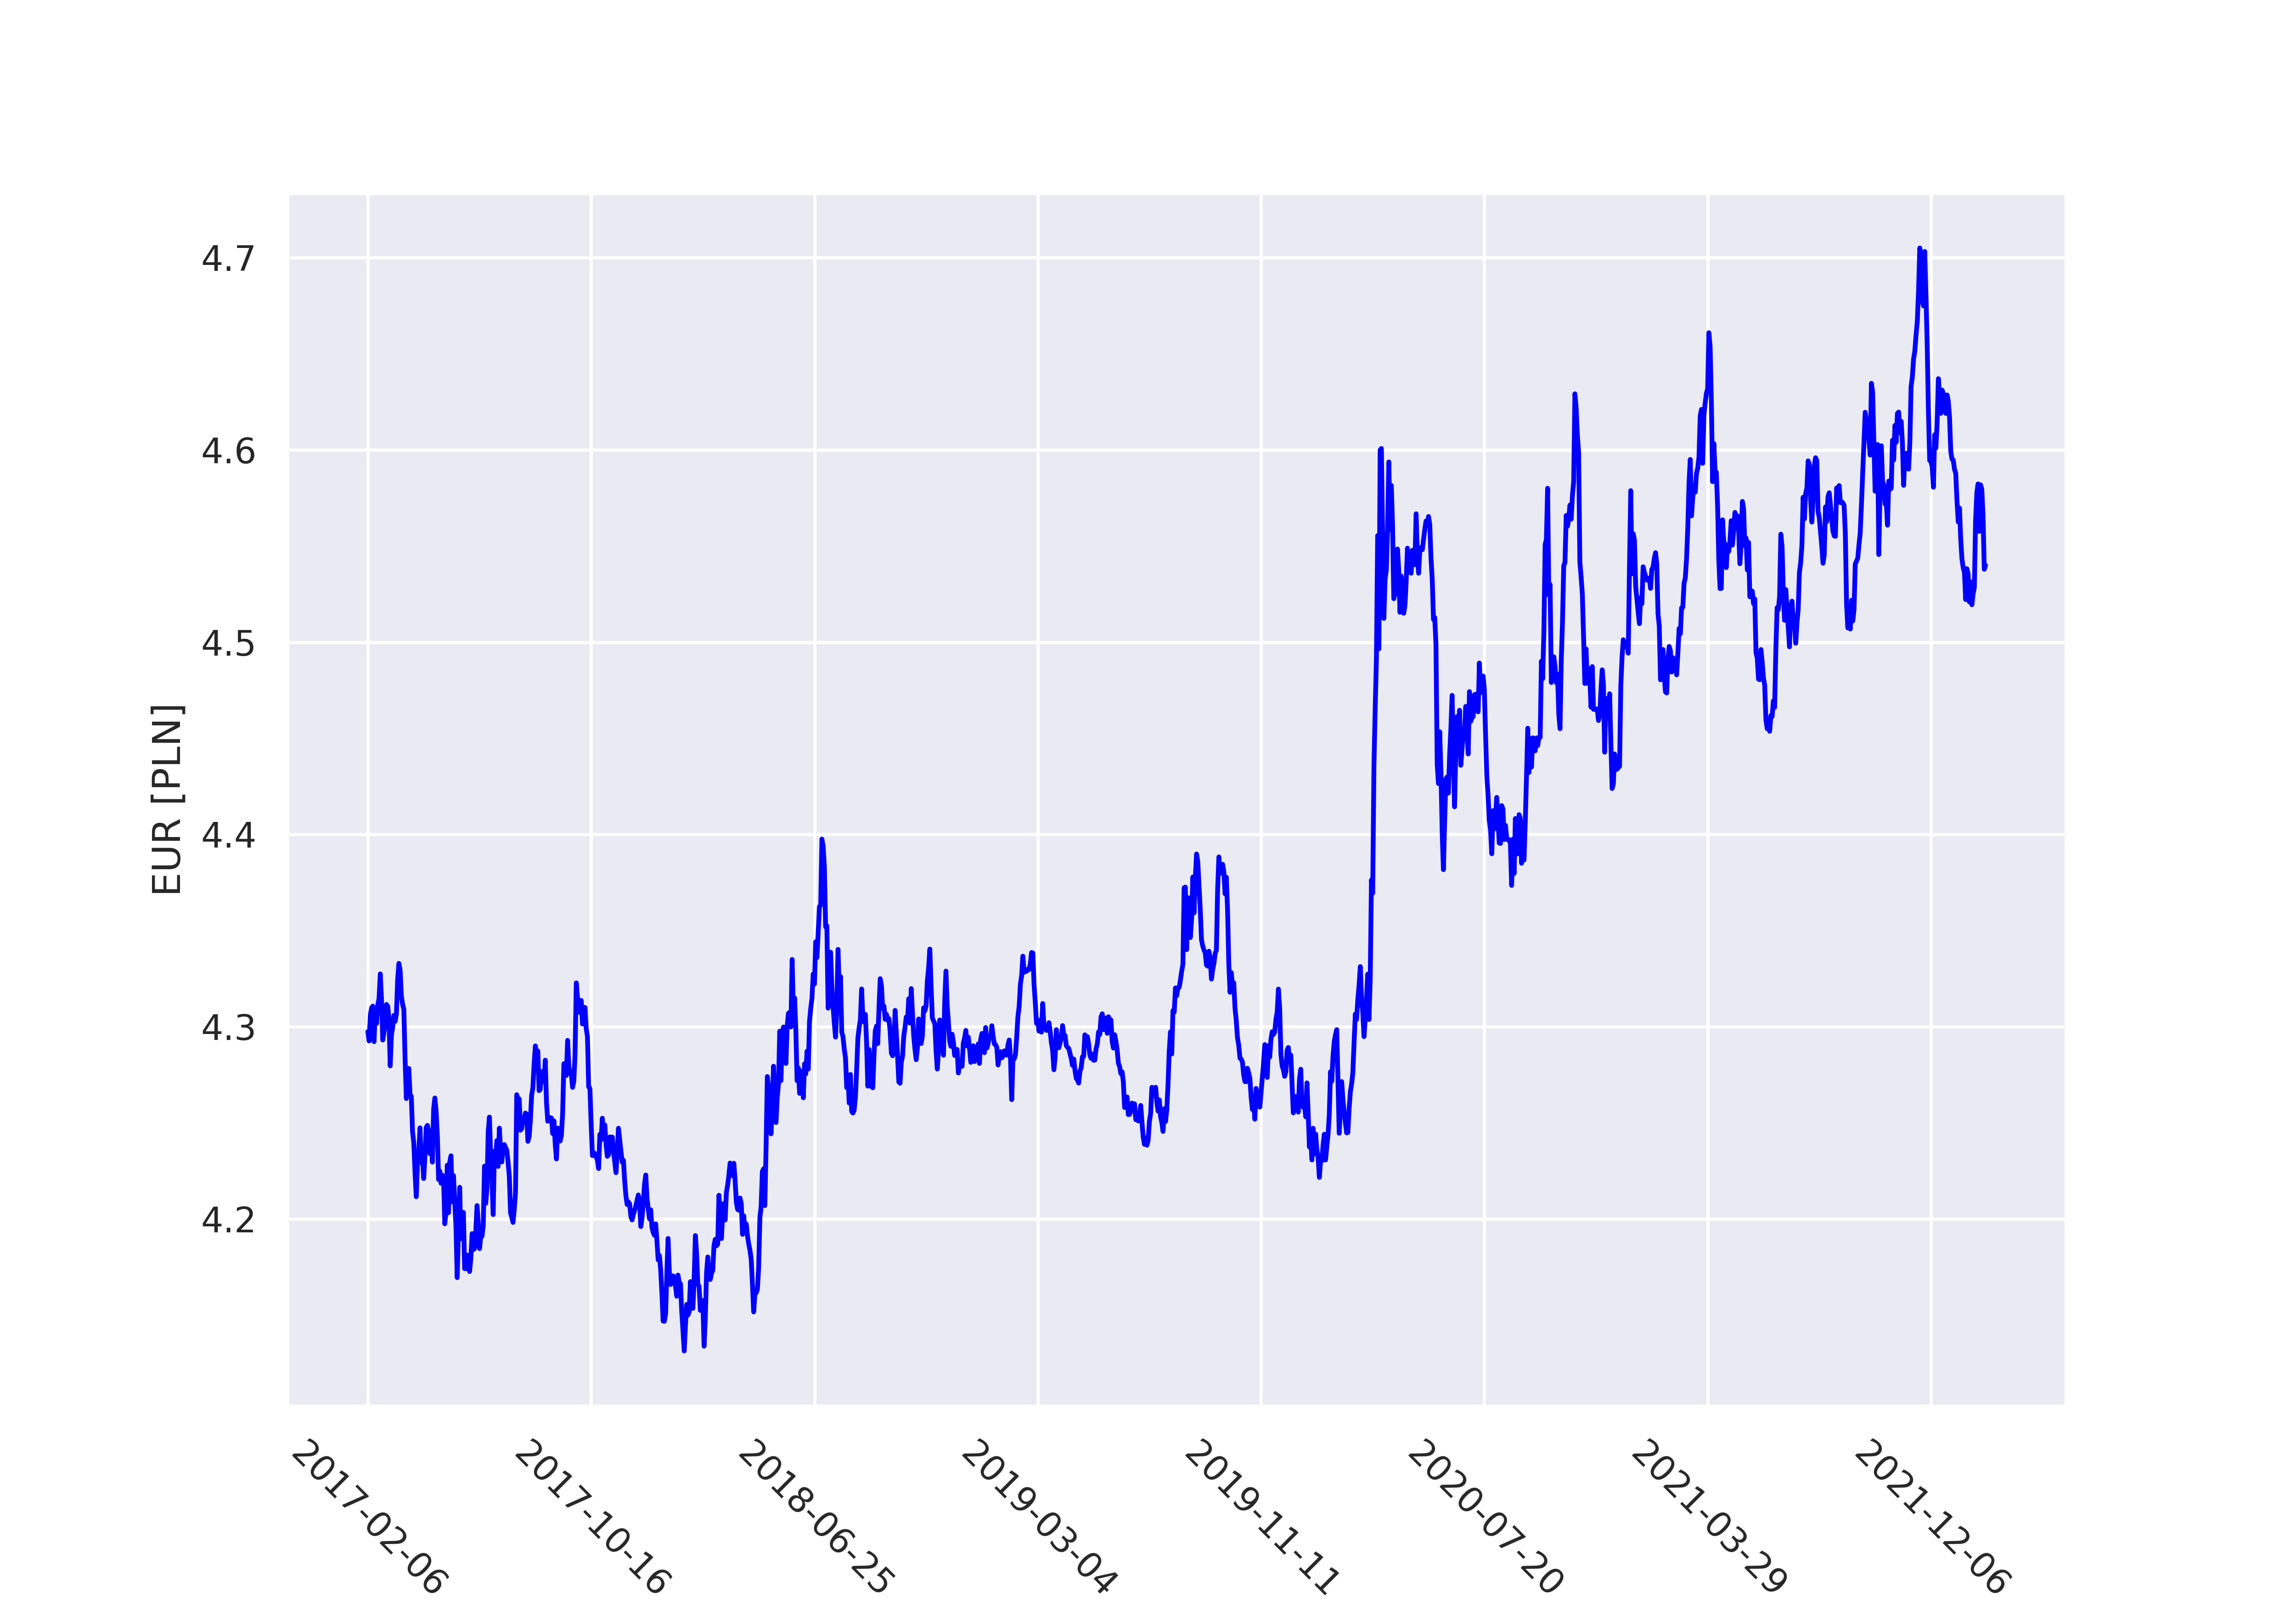
\includegraphics[width=1\textwidth]{data.png}
        \caption{Kurs EUR/PLN w okresie od 2017-02-06 do 2022-02-04}
        \label{fig:dane}
    \end{figure}

    \clearpage

    \section{Statystyki opisowe}

    \subsection{Średnia arytmetyczna}

    $$\overline{x} = \frac{1}{n} \sum_{i=1}^{n} x_{i}$$

    $$\overline{x} \approx 4.36$$

    \subsection{Wariancja}

    $$S^2 = \frac{1}{n} \sum_{i=1}^n\left(x_i - \overline{x}\right)^2$$ 

    $$S^2 \approx 0.02$$

    \subsection{Odchylenie standardowe}

    $$S = \sqrt{S^2}$$ 

    $$S \approx 0.14$$

    \subsection{Mediana}

    Dla posortowanej próby:

    $$med = \text{Q}2 = \begin{cases}
        x_{\frac{n+1}{2}}, & \text{gdy n nieparzyste}\\
        \frac{1}{2}\left(x_{\frac{n}{2}} + x_{\frac{n}{2}+1}\right), & \text{gdy n parzyste}\\
        \end{cases}$$

    $$\text{Q}2 \approx 4.31$$

    \subsection{Kwartyle}

    Pierwszy kwartyl $\text{Q}1$ to mediana grupy obserwacji mniejszych od $\text{Q}2$.

    \noindent Trzeci kwartyl $\text{Q}3$ to mediana grupy obserwacji większych od $\text{Q}2$.

    $$\text{Q}1 \approx 4.26$$
    $$\text{Q}3 \approx 4.50$$

    \subsection{Rozstęp międzykwartylowy}

    $$\text{IQR} = \text{Q}3 - \text{Q}1$$ 

    $$\text{IQR} \approx 0.24$$

    \section{Przygotowanie danych}
        Patrząc na Rysunek \ref{fig:dane}, po danych możemy spodziewać się istnienia pewnego trendu liniowego.
        W celu jego usunięcia skorzystamy z metody różnicowania danych:
        $$
                Y_i = X_i - X_{i-1},
        $$
        gdzie $X_i$ jest i-tą wartością naszego kursu.
        Po takim przetransformowaniu naszych danych uzyskujemy nowy szereg czasowy $Y_i$ z usuniętym trendem liniowym.

    \begin{figure}[H]
        \centering
        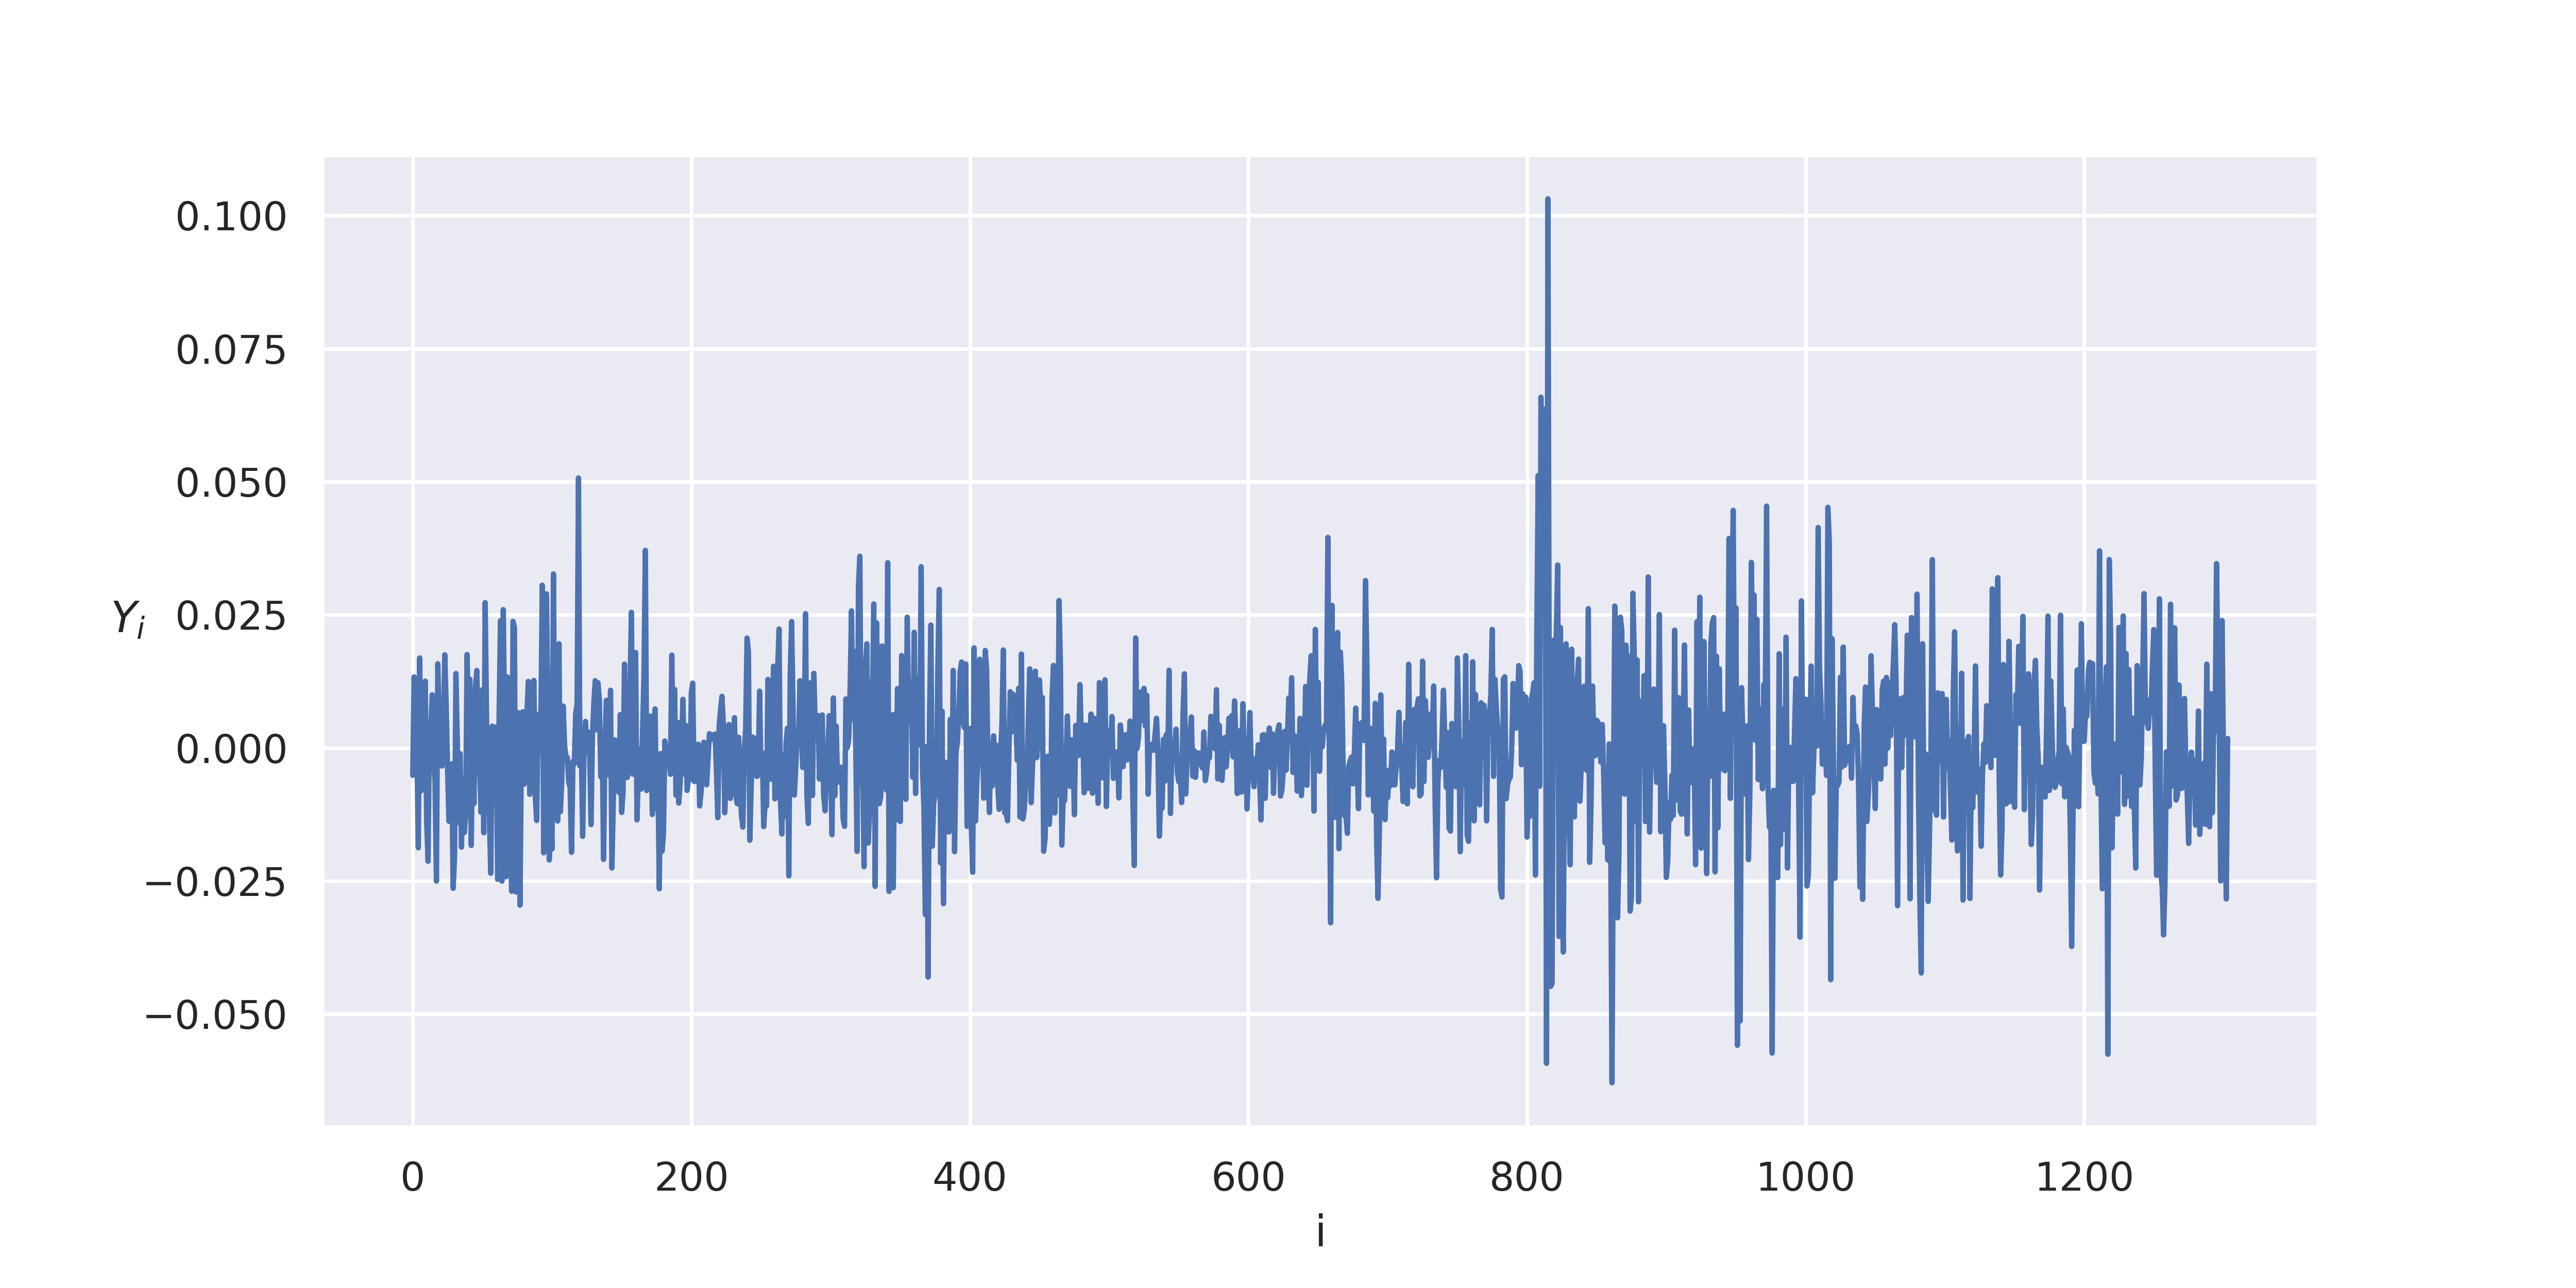
\includegraphics[width=1\textwidth]{trend.png}
        \caption{Dane po zastosowaniu transformacji różnicowej}
        \label{fig:2 Transformacja roznicowa}
    \end{figure}

    \vskip 0.2in
    Oczywiście transformacja danych zmienia ich statystyki opisowe - wartości kilku podstawowych statystyk umieściliśmy w poniższej tabeli:

    \begin{table}[H]
        \centering
        \begin{tabular}{|l|l|l|l|l|l|l|}
        \hline
        mean     & std      & min       & Q1        & Median    & Q3       & max      \\ \hline
        0.000186 & 0.014416 & -0.062600 & -0.007915 & -0.000255 & 0.007535 & 0.103460 \\ \hline
        \end{tabular}
        \caption{Tablica  podstawowych statystyk przetransformowanych danych}
        \label{tab:transform_besic_stats}
    \end{table}

    \vskip 0.2in
    Teraz pokażemy, jak dla naszych danych prezentują się empiryczne funkcje ACF i PACF, dane wzorami:\\

    \begin{itemize}
        \item ACF $$\hat{\rho}(h) = \frac{\hat{\gamma}(h)}{\hat{\gamma}(0)} = \frac{1}{n}\sum_{t=1}^{n-|h|}(x_{t+|h|} - \overline{x})(x_{t} - \overline{x}),$$\\ gdzie $\hat{\gamma}(h)$ - empiryczna funkcja autokowariancji, $n$ - długość próby,\\
        \item PACF $$\alpha(h) = \phi_{hh},$$\\ gdzie $\phi_{hh}$ jest ostatnim współczynnikiem wektora $\phi_{h} = \hat{\Gamma}_{h}^{-1}\hat{\gamma}_{h}$, $\hat{\Gamma}_{h} = \left[\hat{\gamma}(i-j)\right]_{i,j=1}^{h}$.
    \end{itemize}

    \newpage

    \begin{figure}[H]
        \centering
        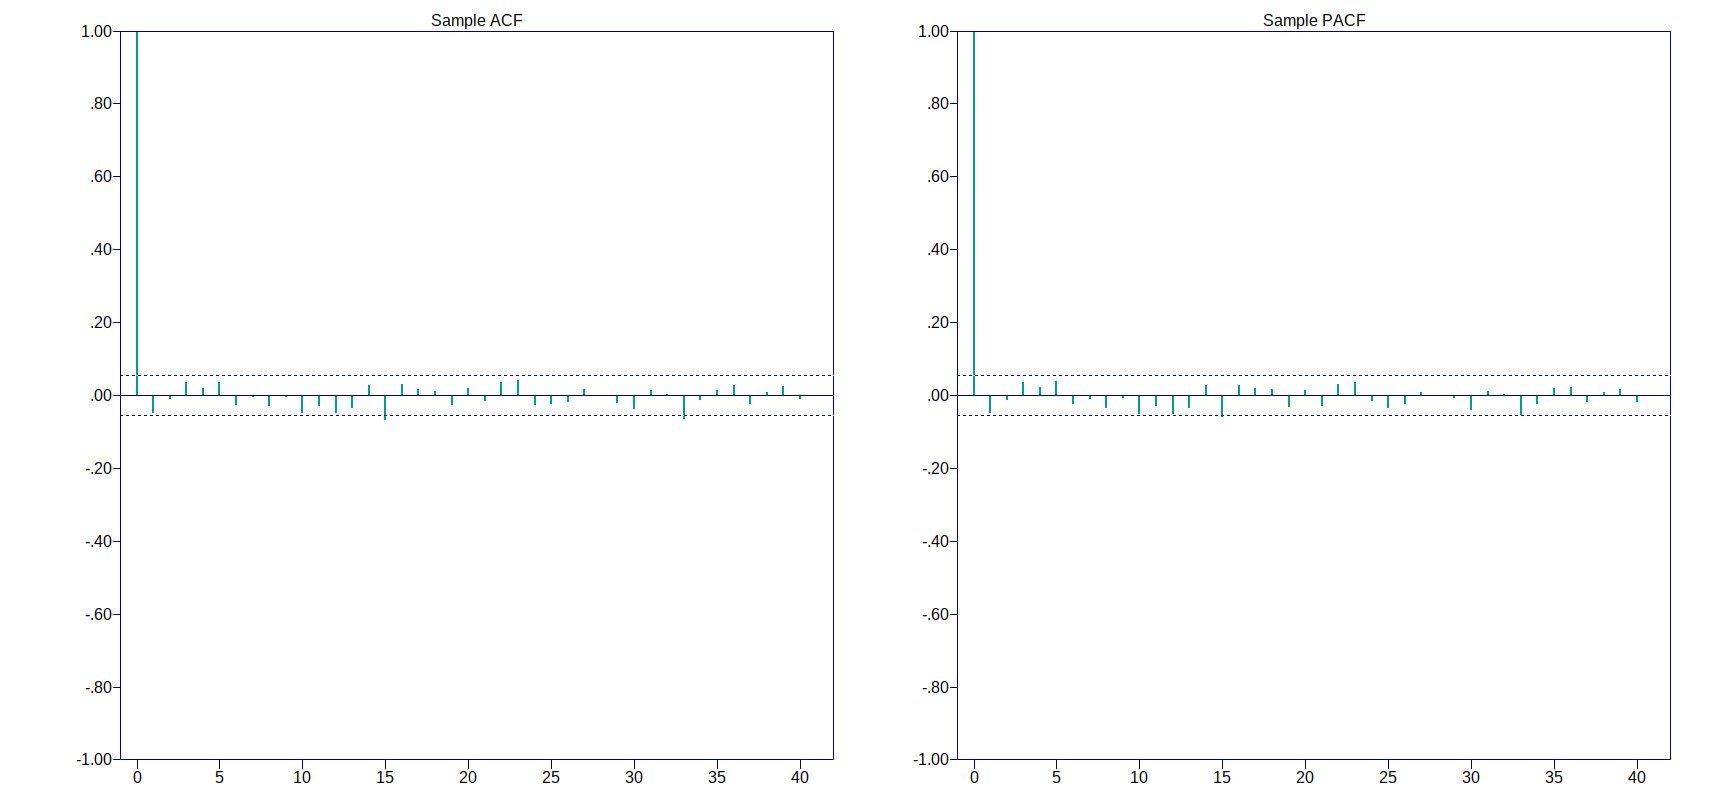
\includegraphics[width=1\textwidth]{acv_pacf.png}
        \caption{Wykresy funkcji ACF i PACF}
        \label{fig:3 ACF_PACF}
    \end{figure}

    \vskip 0.2in 
    Z otrzymanych wykresów widzimy korelację na poziomie 1 tylko dla argumentu 0, w pozostałych przypadkach nasze 
    funkcje oscylują wokół zera. Ponadto teraz średnia dla naszych danych jest stała w czasie i w przybliżeniu wynosi 
    0 - mamy więc dobrze przygotowane dane i możemy już przejść do doboru oraz analizy 
    odpowiedniego modelu ARMA, czyli szeregu autoregresyjnego średniej ruchomej, zdefiniowanego następująco:\\

    \begin{theorem*}
        Szereg czasowy $X_{t}$ jest szeregiem ARMA(p,q), jeśli jest stacjonarny w słabym sensie
        oraz spełnia równanie:\\

        $$
        X_{t} - \phi_1 X_{t-1} - \ldots - \phi_{p} X_{t-p} = Z_{t} + \theta_1 Z_{t-1} + \ldots + \theta_{q} Z_{t-q},
        $$

        gdzie:
        \begin{itemize}
            \item $Z_{t} \sim WN(0, \sigma^2)$,
            \item wielomiany $\phi(z) = 1 - \phi_1 z - \ldots \phi_{p} z^{p}$,
            $\theta(z) = 1 + \theta_1 z + \ldots + \theta_{q} z^{q}$ nie mają wspólnych pierwiastków.
        \end{itemize}
    \end{theorem*}

    \vskip 0.2in
    \section*{Model ARMA(p,q)} 
    Dobieranie parametrów p i q w modelu ARMA opiera się na kryterium informacyjnym Akaike’go. Jest ono oszacowaniem tego, ile informacji tracimy, gdy
    zamiast rzeczywistego modelu wybierzemy rozważany. Wynika stąd, że im mniejsza wartość AIC, tym lepiej dobrany jest nasz model.
    Metoda "Likelyhood", której będziemy używać, opiera się na sprawdzeniu wszystkich kombinacji parametrów p i q modeli ARMA w zadanym przedziale, a następnie wybraniu tych, dla których
    wartość porównywanego kryterium informacyjnego jest najmniejsza. 
    Wykorzystując powyższą metodę otrzymujemy, że model ARMA(6,7) najlepiej estymuje badany szereg czasowy względem kryterium informacyjnego AICC.

    \newpage

    Aby zwizualizować poprawność dobranego przez nas modelu, porównamy empiryczne funkcje ACF i PACF naszych danych
    z teoretycznymi dla wyestymowanego modelu:

    \begin{figure}[H]
        \centering
        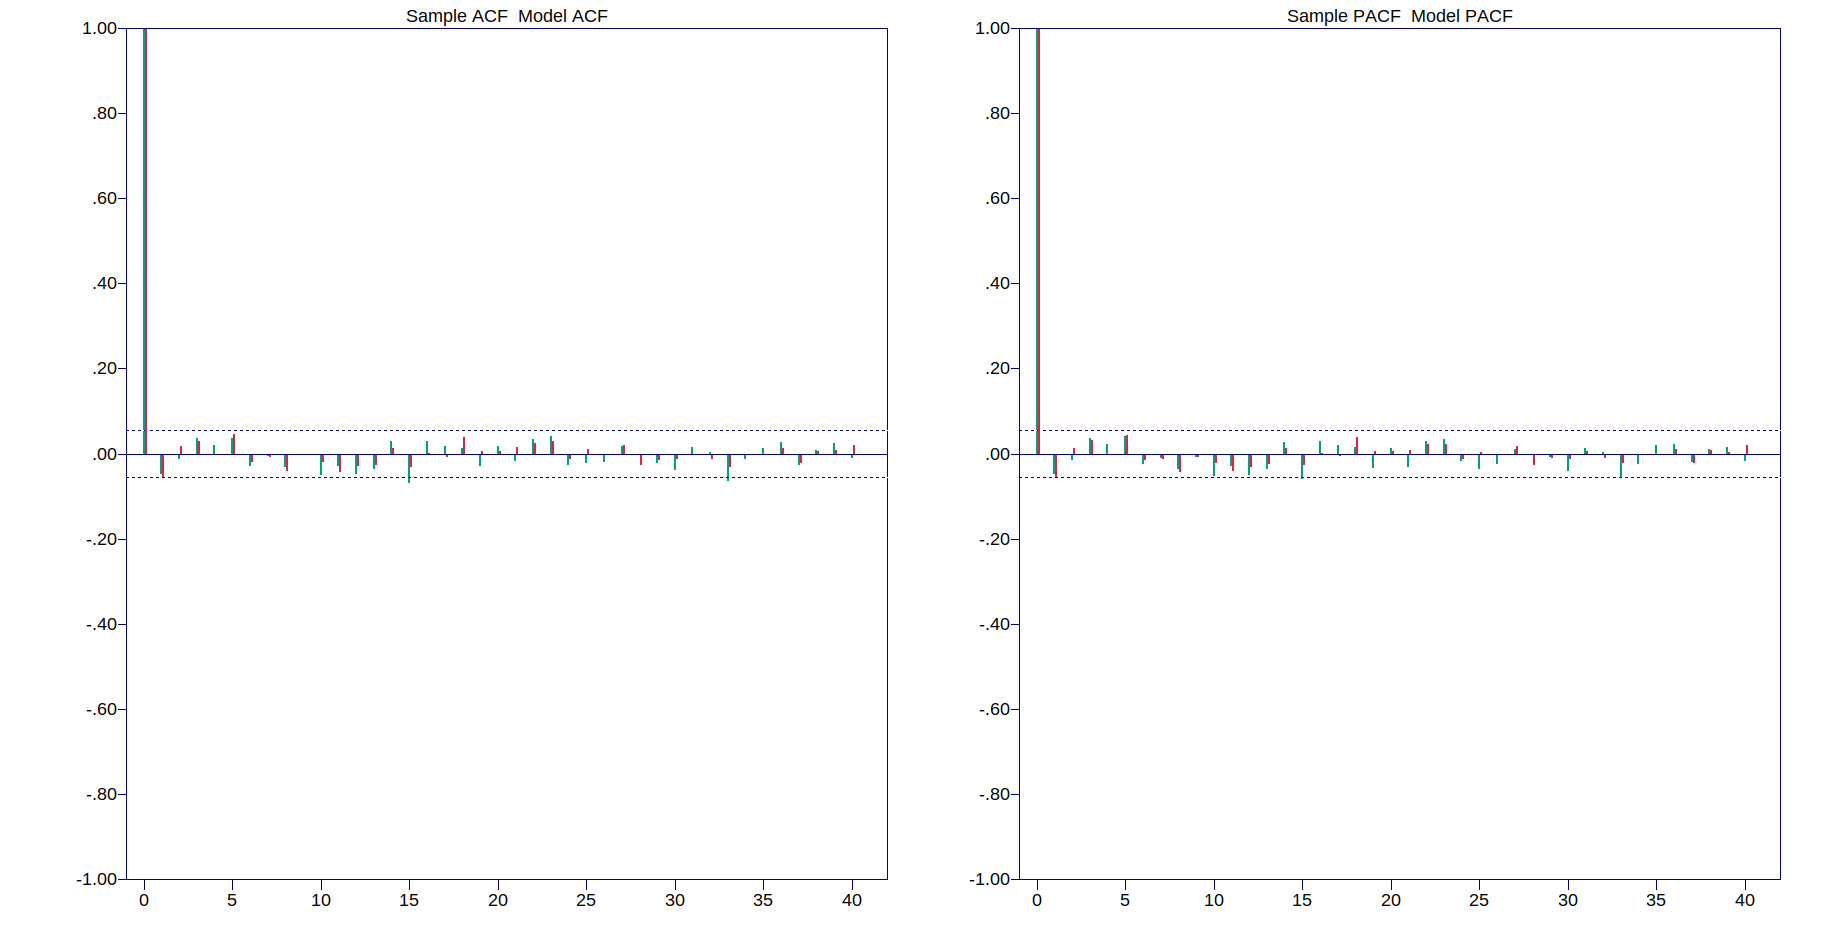
\includegraphics[width=1\textwidth]{acv_pacf_estimeted.png}
        \caption{Porównanie funkcji ACF i PACF teoretycznych z empirycznymi}
        \label{fig:3 acv_pacf_estimeted.png}
    \end{figure}

    \vskip 0.2in
    Widzimy, że w obu przypadkach wykresy funkcji teoretycznych (kolor czerwony) pokrywają się bardzo dobrze z empirycznymi (kolor zielony), 
    co pozwala wnioskować, że model ARMA został przez nas poprawnie dobrany. Możemy zatem przejść do przedstawienia
    wyestymowanych parametrów modelu.


    \subsection*{Estymowane parametry modelu ARMA(p,q)}

    Pierwsza tabela zawiera wartości kolejnych współczynników $\phi_{k}, \; k=1,\ldots,6$ (lewa strona równania w modelu ARMA),
    \begin{table}[H]
        \centering
        \begin{tabular}{|l|l|l|l|l|l|}
        \hline
        $\phi_1$ & $\phi_2$ & $\phi_3$ & $\phi_4$ & $\phi_5$ & $\phi_6$\\
        \hline
        0.178158 & 0.572810 & -0.337375 & 0.632793 & 0.214153 & -0.885537\\
        \hline
        \end{tabular}
        \label{tab:phis_estimated}
        \caption{Parametry $\phi_1,...,\phi_6$}
    \end{table}

    \noindent z drugiej natomiast możemy odczytać wartości współczynników $\theta_{k}, \; k=1,\ldots,7$ (prawa strona równania).

    \begin{table}[H]
        \centering
        \begin{tabular}{|l|l|l|l|l|l|l|}
        \hline
        $\theta_1$ & $\theta_2$ & $\theta_3$ & $\theta_4$ & $\theta_5$ & $\theta_6$ & $\theta_7$\\
        \hline
        -0.235259  & -0.542868  & 0.402289  &  -0.683107 & -0.145044  & 0.889424 & -0.109801\\
        \hline
        \end{tabular}
        \label{tab:thetas_estimated}
        \caption{Parametry $\theta_1,...,\theta_7$}
    \end{table}

    Oprócz tego, istotny dla nas jest również parametr $\sigma^2$, czyli wariancja białego szumu (szereg $Z_t$).
    W naszym przypadku wynosi ona $\sigma^2 = 0.000201$.

    \newpage

    \section*{Analiza residuów}
        W poniższej części zajmiemy się analizą residuów, sprawdzimy czy są nieskorelowane i czy pochodzą z rozkładu normalnego. 
    \begin{figure}[H]
        \centering
        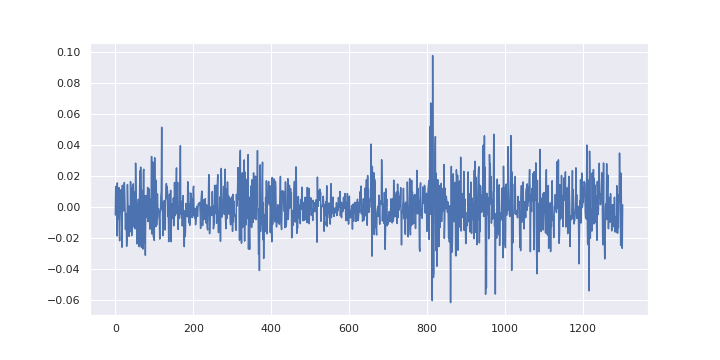
\includegraphics[width=0.85\textwidth]{residuum.png}
        \caption{Wykres residuów}
        \label{fig:residuum}
    \end{figure}
    
    \begin{table}[H]
        \centering
        \begin{tabular}{|l|l|l|l|l|l|l|}
        \hline
        mean     & std      & min       & Q1        & Median    & Q3       & max      \\ \hline
        -0.00000050 & 0.00141866 & -0.05641744 & -0.00832161 & -0.00026310 & 0.00729265 & 0.09383978 \\ \hline
        \end{tabular}
        \caption{Tablica  podstawowych statystyk residuów.}
        \label{tab:resid}
    \end{table}

    Z Tabeli \ref{tab:resid} widzimy, że residua mają średnią bardzo bliską 0.
    Jeśli zaś chodzi o wariancję, możemy zobaczyć jej wyraźną zmianę np. w okolicach osiemsetnej obserwacji, a co za tym 
    idzie, zdecydowanie nie jest ona stała. Teraz chcemy sprawdzić, czy nasze residua są nieskorelowane - w tym celu
    przyjrzymy się wykresom funkcji ACF i PACF.


    \vskip -0.18 in

    \begin{figure}[H]
        \centering
        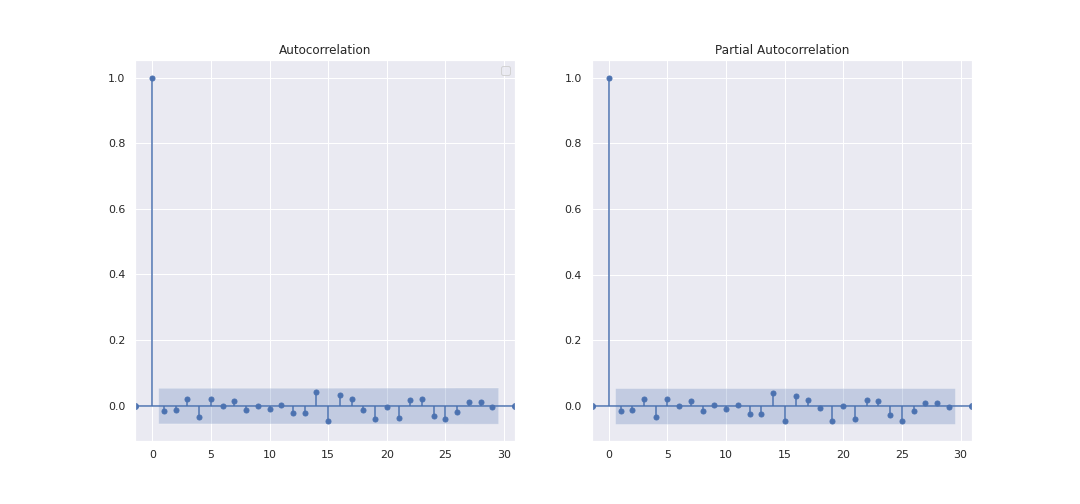
\includegraphics[width=1\textwidth]{res_acf_pacf.png}
        \caption{ACF i PACF residuów}
        \label{fig:res_acf_pacf}
    \end{figure}

    % \newpage
    Analizując powyższe wykresy możemy przypuszczać, że residua są nieskorelowane - aby jednak zweryfikować
    tę hipotezę, przeprowadzamy pięć testów losowości, których wyniki prezentują się następująco:\\

    \begin{itemize}
        \item Ljung - Box: p-value = 0.36053
        \item McLeod - Li: p-value = 0.00000
        \item Turning points: p-value = 0.29299
        \item Diff sign points: p-value = 0.11360
        \item Rank test statistic: p-value = 0.59416
    \end{itemize}

    Z pięciu przeprowadzonych testów, cztery zwracają p-wartość, która na poziomie istotności 0.05
    nie daje podstaw do odrzucenia hipotezy zerowej o braku korelacji między residuami. Widzimy jednak, że 
    test McLeod-Li zwraca p-wartość równą zeru, a zatem musimy odrzucić hipotezę zerową  - wnioskujemy stąd, 
    że nasze residua nie są nieskorelowane. \\

    Następnym krokiem w analizie residuów będzie sprawdzenie, czy pochodzą one z rozkładu normalnego. Najpierw przeprowadzamy test normalności Jarque-Bera. 
    W jego wyniku otrzymujemy p-wartość równą 0, zatem mamy podstawy do odrzucenia hipotezy zerowej o normalności 
    residuów. Chcemy jednak zweryfikować ten wniosek, porównamy więc ich gęstość empiryczną z gęstością teoretyczną rozkładu $\mathcal{N}(0, S^2)$, 
    gdzie $S^2$ jest empiryczną wariancją residuów.

    \begin{figure}[H]
        \centering
        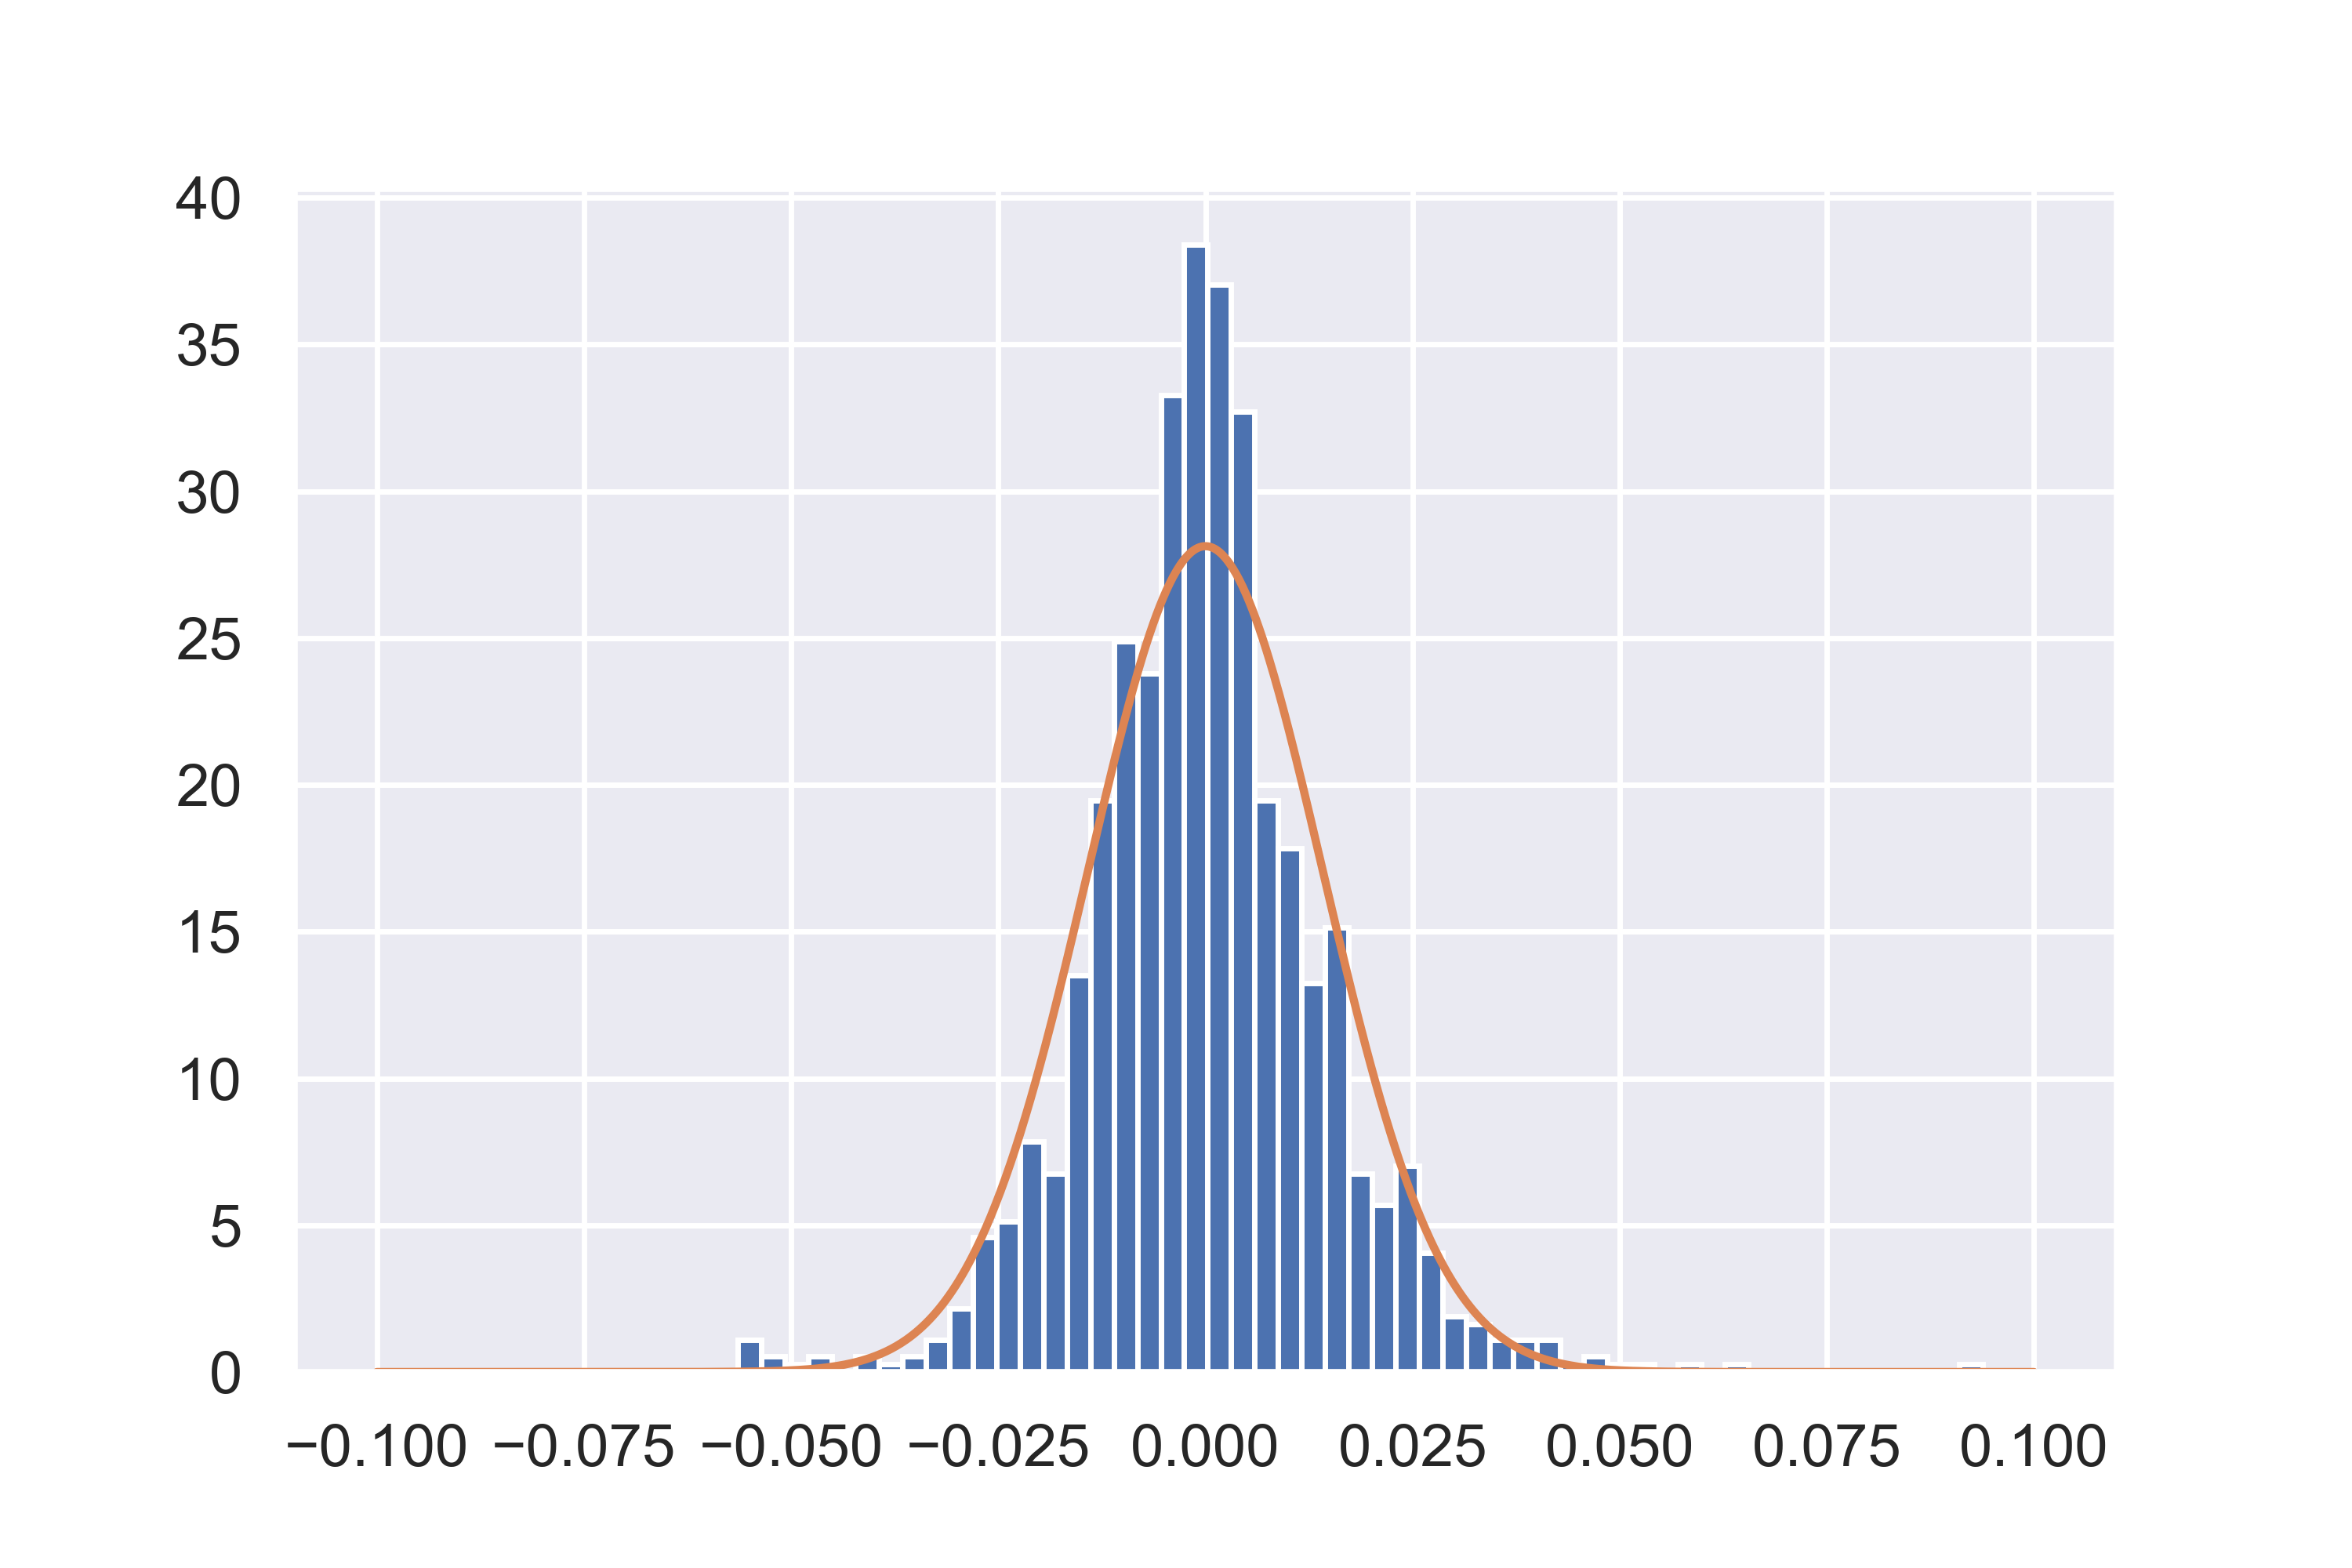
\includegraphics[width=1\textwidth]{res_pdf.png}
        \caption{Porównanie histogramu residuów z gęstością rozkładu $\mathcal{N}(0, S^2)$}
        \label{fig:res_pdf}
    \end{figure}

    Otrzymane wykresy potwierdzają, że powinniśmy odrzucić hipotezę zerową o normalności residuów - 
    różnica między teoretyczną a empiryczną gęstością jest zbyt duża.

    \section*{Podsumowanie}

    Ceny euro na przestrzeni ostatnich czterech lat zdecydowanie rosły, wykazując przy tym trend liniowy. Ich średnia w tym okresie 
    wyniosła 4.36 PLN (bardzo podobnie do mediany, której wartość to 4.31 PLN), natomiast odchylenie 
    od średniej to około 0.14 PLN. Ze względu na liniowy przebieg naszych danych, dokonaliśmy ich różnicowania, w wyniku czego 
    otrzymaliśmy szereg czasowy stacjonarny w słabym sensie, co bardzo dobrze obrazują rysunki \ref{fig:2 Transformacja roznicowa} 
    i \ref{fig:3 ACF_PACF} - widzimy z nich stałą w czasie średnią (równą 0) oraz funkcję autokorelacji niezależną od czasu.
    Tak przetransformowane dane nadawały się już do doboru odpowiedniego modelu ARMA(p, q) oraz jego analizy.
    W tej części sprawozdania posługiwaliśmy się głównie programem \textbf{ITSM}. Przy jego pomocy otrzymaliśmy model o parametrach 
    $p=6$ i $q=7$ (przy wartości AICC równej -7363.83). Mając już dobrany model, dokonaliśmy
    analizy jego residuów, w wyniku której wywnioskowaliśmy, że co prawda mają one średnią $\mu=0$, 
    ale za to ich wariancja jest zmienna w czasie. Dodatkowo residua wykazują pewną korelację między sobą 
    i nie pochodzą z rozkładu normalnego. 
\end{document}